\documentclass[11pt,letterpaper]{article}
\usepackage[lmargin=1in,rmargin=1in,tmargin=1in,bmargin=1in]{geometry}
\usepackage{../style/homework}
\usepackage{../style/commands}
\setbool{quotetype}{true} % True: Side; False: Under
\setbool{hideans}{false} % Student: True; Instructor: False

% -------------------
% Content
% -------------------
\begin{document}

\homework{18: Due 12/06}{True optimization is the revolutionary contribution of modern research to decision processes.}{George Dantzig}

% Problem 1
\problem{10} As accurately as possible, sketch the feasible region given by the following maximization problem on the plot below: \par
	\begin{minipage}[b]{0.3\textwidth}
	\[
	\begin{aligned}
	\text{max } z= 4x_1& + 6x_2 \\
	-x_1 + 5x_2&\leq 5 \\
	x_1 + x_2&\leq 11 \\
	x_1, x_2&\geq 0 \\
	x_1&\leq 7
	\end{aligned}
	\]
	\end{minipage}\begin{minipage}{0.69\textwidth}
	\[
	\fbox{
	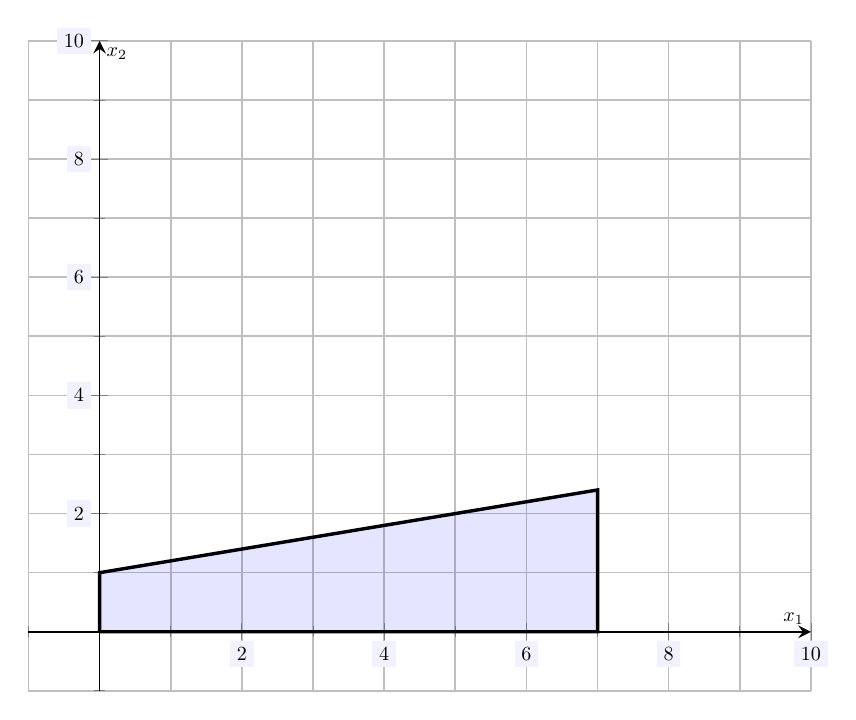
\begin{tikzpicture}[scale=1.45,every node/.style={scale=0.5}]
	\begin{axis}[
	grid=both,
	axis lines=middle,
	ticklabel style={fill=blue!5!white},
	xmin= -1, xmax=10,
	ymin= -1, ymax=10,
	xtick={0,2,4,6,8,10},
	ytick={0,2,4,6,8,10},
	minor tick = {-1,0,1,...,10},
	xlabel=\(x_1\),ylabel=\(x_2\),
	]
%	\addplot[line width=0.03cm, domain= -2:10] (x, 11 - x);
%	\addplot[line width=0.03cm, domain= -2:10] (x, 1/5*x + 1);
%	\draw[line width=0.03cm] (7, -2) -- (7,10);
	\draw[line width=0.01cm,fill= blue,opacity=0.1] (0,0) -- (0,1) -- (7,12/5) -- (7,0) -- (0,0);
	\draw[line width=0.03cm] (0,0) -- (0,1) -- (7,12/5) -- (7,0) -- (0,0);
	\end{axis}
	\end{tikzpicture}
	}
	\]
	\end{minipage} \pspace
Is this region nonempty? Is this region bounded or unbounded? Solve this maximization problem. \pspace

\sol `Solving' $-x_1 + 5x_2 \leq 5$ for $x_2$, we obtain $x_2 \leq \frac{1}{5}\,x_1 + 1$. The line $x_2= \frac{1}{5}\,x_1 + 1$ has $y$-intercept 1 and slope $\frac{1}{5}$. Because $x_2 \leq \frac{1}{5}\,x_1 + 1$, we shade below this line. `Solving' $x_1 + x_2 \leq 11$ for $x_2$, we obtain $x_2 \leq 11 - x_1$. The line $x_2= 11 - x_1$ has $y$-intercept 11 and slope $-1$. Because $x_2 \leq 11 - x_1$, we shade below this line. The line $x_1= 7$ is a vertical line with $x_1= 7$ for all points on the line. Because $x_1 \leq 7$, we shade to the left of this line. The line $x_1= 0$ is the $y$-axis. Because $x_1 \geq 0$, we need shade to the right of the $y$-axis. The line $x_2= 0$ is the $x$-axis. Because $x_2 \geq 0$, we need shade above the $x$-axis. [Note: Together, the inequalities $x_1, x_2 \geq 0$ simply state that the region must be in Quadrant~I.] Sketching this above, we see that we need the intersection of $x_2= \frac{1}{5}\,x_1 + 1$ and $x_1= 7$. But if $x_1= 7$, then $x_2= \frac{1}{5} \cdot 7 + 1= \frac{12}{5}$. Therefore, the lines intersect at $\left( 7, \frac{12}{5} \right)$. Putting all this information together, we obtain the region shaded above. \pspace

This region is clearly nonempty. Because we can easily draw a `ball' around the region, the region is also bounded. The function $z= 4x_1 + 6x_2$ is linear. Therefore, the Fundamental Theorem of Linear Programming states that the function $z$ has a maximum and minimum value on this region and that they occur at a corner point. The corner points are $(0,0)$, $(0,1)$, $\big(7, \frac{12}{5} \big)$, and $(7, 0)$. Evaluating $z$ at these points, we find $z(0,0)= 0$, $z(0,1)= 0 + 6= 6$, $z\big(7, \frac{12}{5} \big)= 28 + \frac{72}{5}= \frac{212}{5}$, and $z(7,0)= 28 + 0= 28$. Clearly, the maximum value of $z$ on this region is $\frac{212}{5}$ and occurs at $(x_1, x_2)= \big(7, \frac{12}{5} \big)$. 



\newpage



% Problem 2
\problem{10} As accurately as possible, sketch the feasible region given by the following maximization problem on the plot below: \par
	\begin{minipage}[b]{0.3\textwidth}
	\[
	\begin{aligned}
	\text{min } z= 4x_1& + 6x_2 \\
	2x_1 + x_2&\geq 6 \\
	2x_1 + 3x_2&\geq 10 \\
	x_1, x_2&\geq 0
	\end{aligned}
	\]
	\end{minipage}\begin{minipage}{0.69\textwidth}
	\[
	\fbox{
	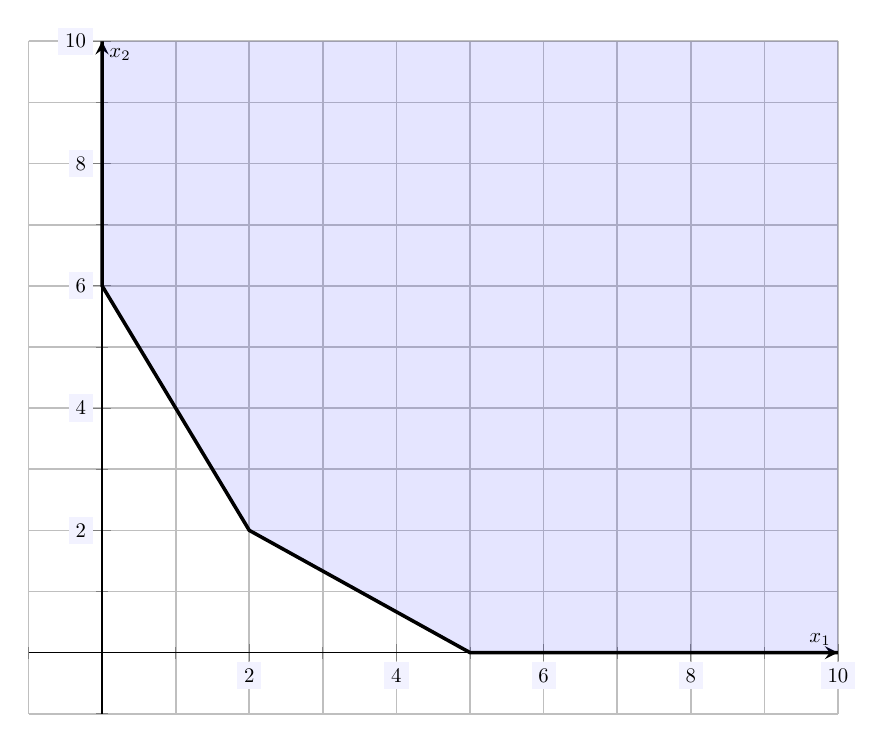
\begin{tikzpicture}[scale=1.5,every node/.style={scale=0.5}]
	\begin{axis}[
	grid=both,
	axis lines=middle,
	ticklabel style={fill=blue!5!white},
	xmin= -1, xmax=10,
	ymin= -1, ymax=10,
	xtick={0,2,4,6,8,10},
	ytick={0,2,4,6,8,10},
	minor tick = {-1,0,1,...,10},
	xlabel=\(x_1\),ylabel=\(x_2\),
	]
%	\addplot[line width=0.03cm, domain= -1:10] (x,6-2*x);
%	\addplot[line width=0.03cm, domain= -1:10] (x,10/3-2/3*x);
	\draw[line width=0.01cm,fill= blue,opacity=0.1] (0,10) -- (0,6) -- (2,2) -- (5,0) -- (10,0) -- (10,10) -- (0,10);
	\draw[line width=0.03cm] (0,10) -- (0,6) -- (2,2) -- (5,0) -- (10,0);
	\end{axis}
	\end{tikzpicture}
	}
	\]
	\end{minipage} \pspace
Is this region nonempty? Is this region bounded or unbounded? Solve this minimization problem. \pspace

\sol `Solving' for $x_2$ in $2x_1 + x_2 \geq 6$, we obtain $x_2 \geq 6 - 2x_1$. The line $x_2= 6 - 2x_1$ has $y$-intercept 6 and slope $-2$. Because $x_2 \geq 6 - 2x_1$, we shade above the line. `Solving' for $x_2$ in $2x_1 + 3x_2 \geq 10$, we obtain $x_2 \geq \frac{10}{3} - \frac{2}{3}\,x_1$. The line $x_2= \frac{10}{3} - \frac{2}{3}\,x_1$ has $y$-intercept $\frac{10}{3}$ and slope $-\frac{2}{3}$. Because $x_2 \geq \frac{10}{3} - \frac{2}{3}\,x_1$, we shade above the line. The line $x_1= 0$ is the $y$-axis. Because $x_1 \geq 0$, we need shade to the right of the $y$-axis. The line $x_2= 0$ is the $x$-axis. Because $x_2 \geq 0$, we need shade above the $x$-axis. [Note: Together, the inequalities $x_1, x_2 \geq 0$ simply state that the region must be in Quadrant~I.] Sketching this above, we see we need the intersection of $x_2= 6 - 2x_1$ and $x_2= \frac{10}{3} - \frac{2}{3}\,x_1$. This gives $6 - 2x_1= \frac{10}{3} - \frac{2}{3}\,x_1$. Multiplying both sides by 3, we obtain $18 - 6x_1= 10 - 2x_1$. But then $4x_1= 8$ so that $x_1= 2$. But then $x_2= 6 - 2(2)= 6 - 2= 2$. Therefore, the lines intersect at $(x_1, x_2)= (2, 2)$. We also need the $x$-intercept of $x_2= \frac{10}{3} - \frac{2}{3}\,x_1$. But then $0= \frac{10}{3} - \frac{2}{3}\,x_1$ so that $x_1= 5$, i.e. the $x$-intercept is $(x_1, x_2)= (5, 0)$. Putting all this information together yields the region shaded in the graph above. \pspace

Clearly, the region is nonempty. Because there is no `ball' which encloses the entire region, the region is unbounded. But then the Fundamental Theorem of Linear Programming does not apply. However, increasing either $x_1$ or $x_2$ increases $z$. Because we can always increase $x_1$ or $x_2$ and stay within the region, $z$ does not have a maximum on this region. However, vice versa, decreasing $x_1$ or $x_2$ decreases $z$. Because the region is `bounded from below', the function has a minimum and must occur at a corner point. The corner points are $(0,6)$, $(2,2)$, and $(5,0)$. Evaluating $z$ at these points, we find $z(0,6)= 0 + 36= 36$, $z(2,2)= 8 + 12= 20$, and $z(5,0)= 20 + 0= 20$. Therefore, the minimum value is 20 and occurs at $(2, 2)$ or $(5,0)$ (actually, along the line $x_2= \frac{10}{3} - \frac{2}{3}\,x_1$). 


\end{document}